%%
%% copyright quintard julien
%%
%% kaneton
%%
%% design.tex
%%
%% path          /home/ultima/g/kaneton/view/cursus/schedule
%%
%% made by mycure
%%         quintard julien   [quinta_j@epita.fr]
%%
%% started on    Fri Feb  4 15:10:05 2005   mycure
%% last update   Fri Jan  6 02:45:24 2006   cedric
%%

%
% template
%

%
% ---------- header -----------------------------------------------------------
%
% project       kaneton
%
% license       kaneton
%
% file          /home/mycure/kaneton/view/template/paper.tex
%
% created       julien quintard   [wed may 16 18:17:37 2007]
% updated       julien quintard   [fri oct  5 07:00:45 2007]
%

%
% class
%

\documentclass[10pt,a4wide]{article}

%
% packages
%

\usepackage[english]{babel}
\usepackage[T1]{fontenc}
\usepackage{a4wide}
\usepackage{fancyheadings}
\usepackage{multicol}
\usepackage{indentfirst}
\usepackage{graphicx}
\usepackage{color}
\usepackage{xcolor}
\usepackage{verbatim}
\usepackage{aeguill}

\pagestyle{fancy}

\setlength{\footrulewidth}{0.3pt}
\setlength{\parindent}{0.3cm}
\setlength{\parskip}{2ex plus 0.5ex minus 0.2ex}

%
% logos
%

\newcommand{\logos}
  {
    \begin{center}
      
\includegraphics[scale=0.8]{\path/logo/kaneton.pdf}
    \end{center}
  }

%
% prototype
%

\newcommand\prototype[2]{
  \begin{tabular}{p{0.2cm}p{13.8cm}}
  & #1
  \end{tabular}

  \begin{tabular}{p{1cm}p{13cm}}
  & #2
  \end{tabular}}

%
% verbatim stuff
%

\definecolor{verbatimcolor}{rgb}{0.00,0.40,0.00}

\makeatletter

\renewcommand{\verbatim@font}
  {\ttfamily\footnotesize\selectfont}

\def\verbatim@processline{
  {\color{verbatimcolor}\the\verbatim@line}\par
}

\makeatother

%
% header
%

\rhead{}
\rfoot{\scriptsize{The kaneton microkernel project}}

\date{\scriptsize{\today}}


%
% header
%

\lhead{\scriptsize{The kaneton project scheduling}}

%
% title
%

\title{The kaneton microkernel project}

%
% authors
%

\author{\small{Julien Quintard}}

%
% document
%

\begin{document}

%
% title
%

\maketitle

%
% --------- text --------------------------------------------------------------
%

\begin{multicols}{2}


%
% overview
%

\section{Overview}

The kaneton microkernel project's goal is to lead students to understand
what really is an operating system and more precisely a kernel.

Every group, composed of two students, will have to develop parts of
the kaneton microkernel.

To simplify the project, each group receives a development environment
containing everything necessary to start the project including a
working microkernel base, documentation, assignments etc..

The project comes with two fundamental courses:

\begin{itemize}
  \item
    \textbf{Kernel}: this course explores the kernels internals including
    microkernel architectures, memory management, processes and threads,
    synchronisation, communications, and complete case studies.
  \item
    \textbf{MIPS architecture}: this course is dedicated to the MIPS internal
    architecture although this course actually explains modern microprocessors
    concepts: pipelining, optimizations, caches etc..
\end{itemize}

The whole kaneton project is subdivided into parts:

\begin{itemize}
  \item
    \textbf{k0}: this project will be entirely developed during a
    special coding session of about 6 hours and under the teachers'
    supervisation. This project consists in an introduction to the
    MIPS external architecture: basic memory management model,
    MIPS assembly language, development tools etc..
  \item
    \textbf{k1}: this project will lead the students to an higher abstraction
    level. The goal of the project is to develop the segment manager to be
    able to manage physical memory and the architecture-dependent part of the
    region manager to be able to control the virtual memory. This project
    is \textbf{two weeks} long.
  \item
    \textbf{k2}: this project introduces the interrupts management and
    the driver development. Indeed, the student will have to install
    everything necessary to handle interrupts. Then, some drivers will
    be developed including the keyboard, the timer and a demonstration shell.
    This project is \textbf{two weeks} long.
  \item
    \textbf{k3}: the students will have to provide everything necessary
    to handle execution contexts. Indeed, the student will have to
    develop the scheduler but also to implement the context switchs from
    the microprocessor point of view. This project is \textbf{three weeks}
    long
  \item
    \textbf{k4}: this project introduces the communication into the
    microkernel. Indeed, the students will have to provide some
    communication primitives including sychronous and asynchronous
    functions as well as blocking and non-blocking functions. This project
    is \textbf{two weeks} long.
  \item
    \textbf{kn}: this project is a free one. Each group has to choose the
    subject of this project, to design, to implement and to document
    the project.
\end{itemize}

%
% arch-MIPS
%

\section{arch-MIPS}

\textit{Name}: \textbf{MIA}

\textit{Hours}: \textbf{30 hours} divided into \textbf{10 sessions}

\textit{Professor}: \textbf{Julien Quintard}

This course is intended to give students a complete view of how a RISC
microprocessor works and what choices the designers made to build the
future modern microprocessors.

Below are listed the concepts studied in this course:

\begin{itemize}
  \item
    External architecture: we will study the instructions set,
    the memory management model etc..
  \item
    Pipeline: we will study the MIPS pipeline, its inherent problems
    and limitations. Advanced pipelines will also be studied.
  \item
    Compiler optimisations: we will study the different direct assembly
    source code optimisations: rescheduling, software pipelining etc..
  \item
    Memory: we will study the bus used on the MIPS processor and
    the different cache management techniques.
\end{itemize}

The list below details the different sessions for the MIPS architecture
course:

\begin{enumerate}
  \item
    Course presentation, MIPS history, introduction to MIPS external
    architecture: registers and instructions set. Introduction to
    instruction formats and to inherent limitations. (3 hours)
  \item
    End of instruction formats introduction, explanations of architecture
    designers choices: MIXs and Amdhal Rule. Some exercises to practice.
    Introduction to MIPS architecture addressing and to MIPS pipeline.
    (3 hours)
  \item
    Introduction to MIPS spirit and to its pipeline. Moore Law and
    pipeline rules. Introduction to different pipeline representations:
    simplified and detailed. Some exercises to pratice these representations.
    (3 hours)
  \item
    We will study in this session the next instruction address computation
    problem and the delay slot. Then, study of branch instruction and their
    problems and limitations. Some exercises to pratice. (3 hours)
  \item
    Complete study of instruction dependencies. Some exercise to practice.
    (3 hours)
  \item
    Partial exam correction. Introduction to optimisations. (3 hours)
  \item
    Study of different optimisations used by compilers. Study of
    advanced pipelines: superpipeline, superscalar pipelines etc.. (3 hours)
  \item
    Introduction to the Pi-Bus used by the MIPS microprocessor. Then complete
    study of memory including cache management. (3 hours)
  \item
    End of memory course. Some exercises to practice. (3 hours)
  \item
    Revisions for the final exam. (3 hours)
\end{enumerate}

%
% kernel
%

\section{kernel}

\textit{Name}: \textbf{KER}

\textit{Hours}: \textbf{20 hours} divided into \textbf{10 sessions}

\textit{Professor}: \textbf{Cedric Aubouy}

This course is intended to give the students a general overview of
kernel internals and its problematics.

Below are listed the studied notions:

\begin{itemize}
  \item
    Understand how kernel developpement evolves and why, receive a
    minimal general culture on kernel internals and history.
  \item
    We will see how to manage and share common resources (memory,
    execution time) with increasing constraints and needs.
  \item
    In each aspect of the kernel studies, students will learn the
    common security issues and how to solve them.
  \item
    The common kernel design issues will be totally understood by the
    students and they will be able to build their own design.
  \item
    The course aims at giving the students a precise idea of how it
    works inside, thus giving them the ability to fully understand
    the kaneton project.
\end{itemize}

The list below details the different sessions for the kernel course.

\begin{enumerate}
  \item
    \textbf{Microkernel}: quick introduction to the courses. Overview
    of kernel history and trends. Birth and evolution of microkernels, their
    fundamentals. (2 hours)
  \item
    \textbf{Memory management}: hardware base of memory management. What
    kind of resulting constraints? Physcical and virtual memory
    management. (2 hours)
  \item
    \textbf{Processes \& threads}: current kernels manage simultaneous
    executions. What kind of solutions to handle them? (2 hours)
  \item
    \textbf{Synchronisation}: concurrent access to shared resources is a
    common problem in all levels of multithreaded kernels. How to resolve it,
    famous case studies. (2 hours)
  \item
    \textbf{Communication (IPC)}: quick overview of communications forms
    from signals to message passing. New problems in the security and shape of
    IPC, introduced by the microkernel design. (2 hours)
  \item
    \textbf{Case studies}: studies on L4, Mach, Hurd and Chorus. (4 x 2 hours)
\end{enumerate}

\end{multicols}

% XXX
%\begin{figure}[h]
%\centerline{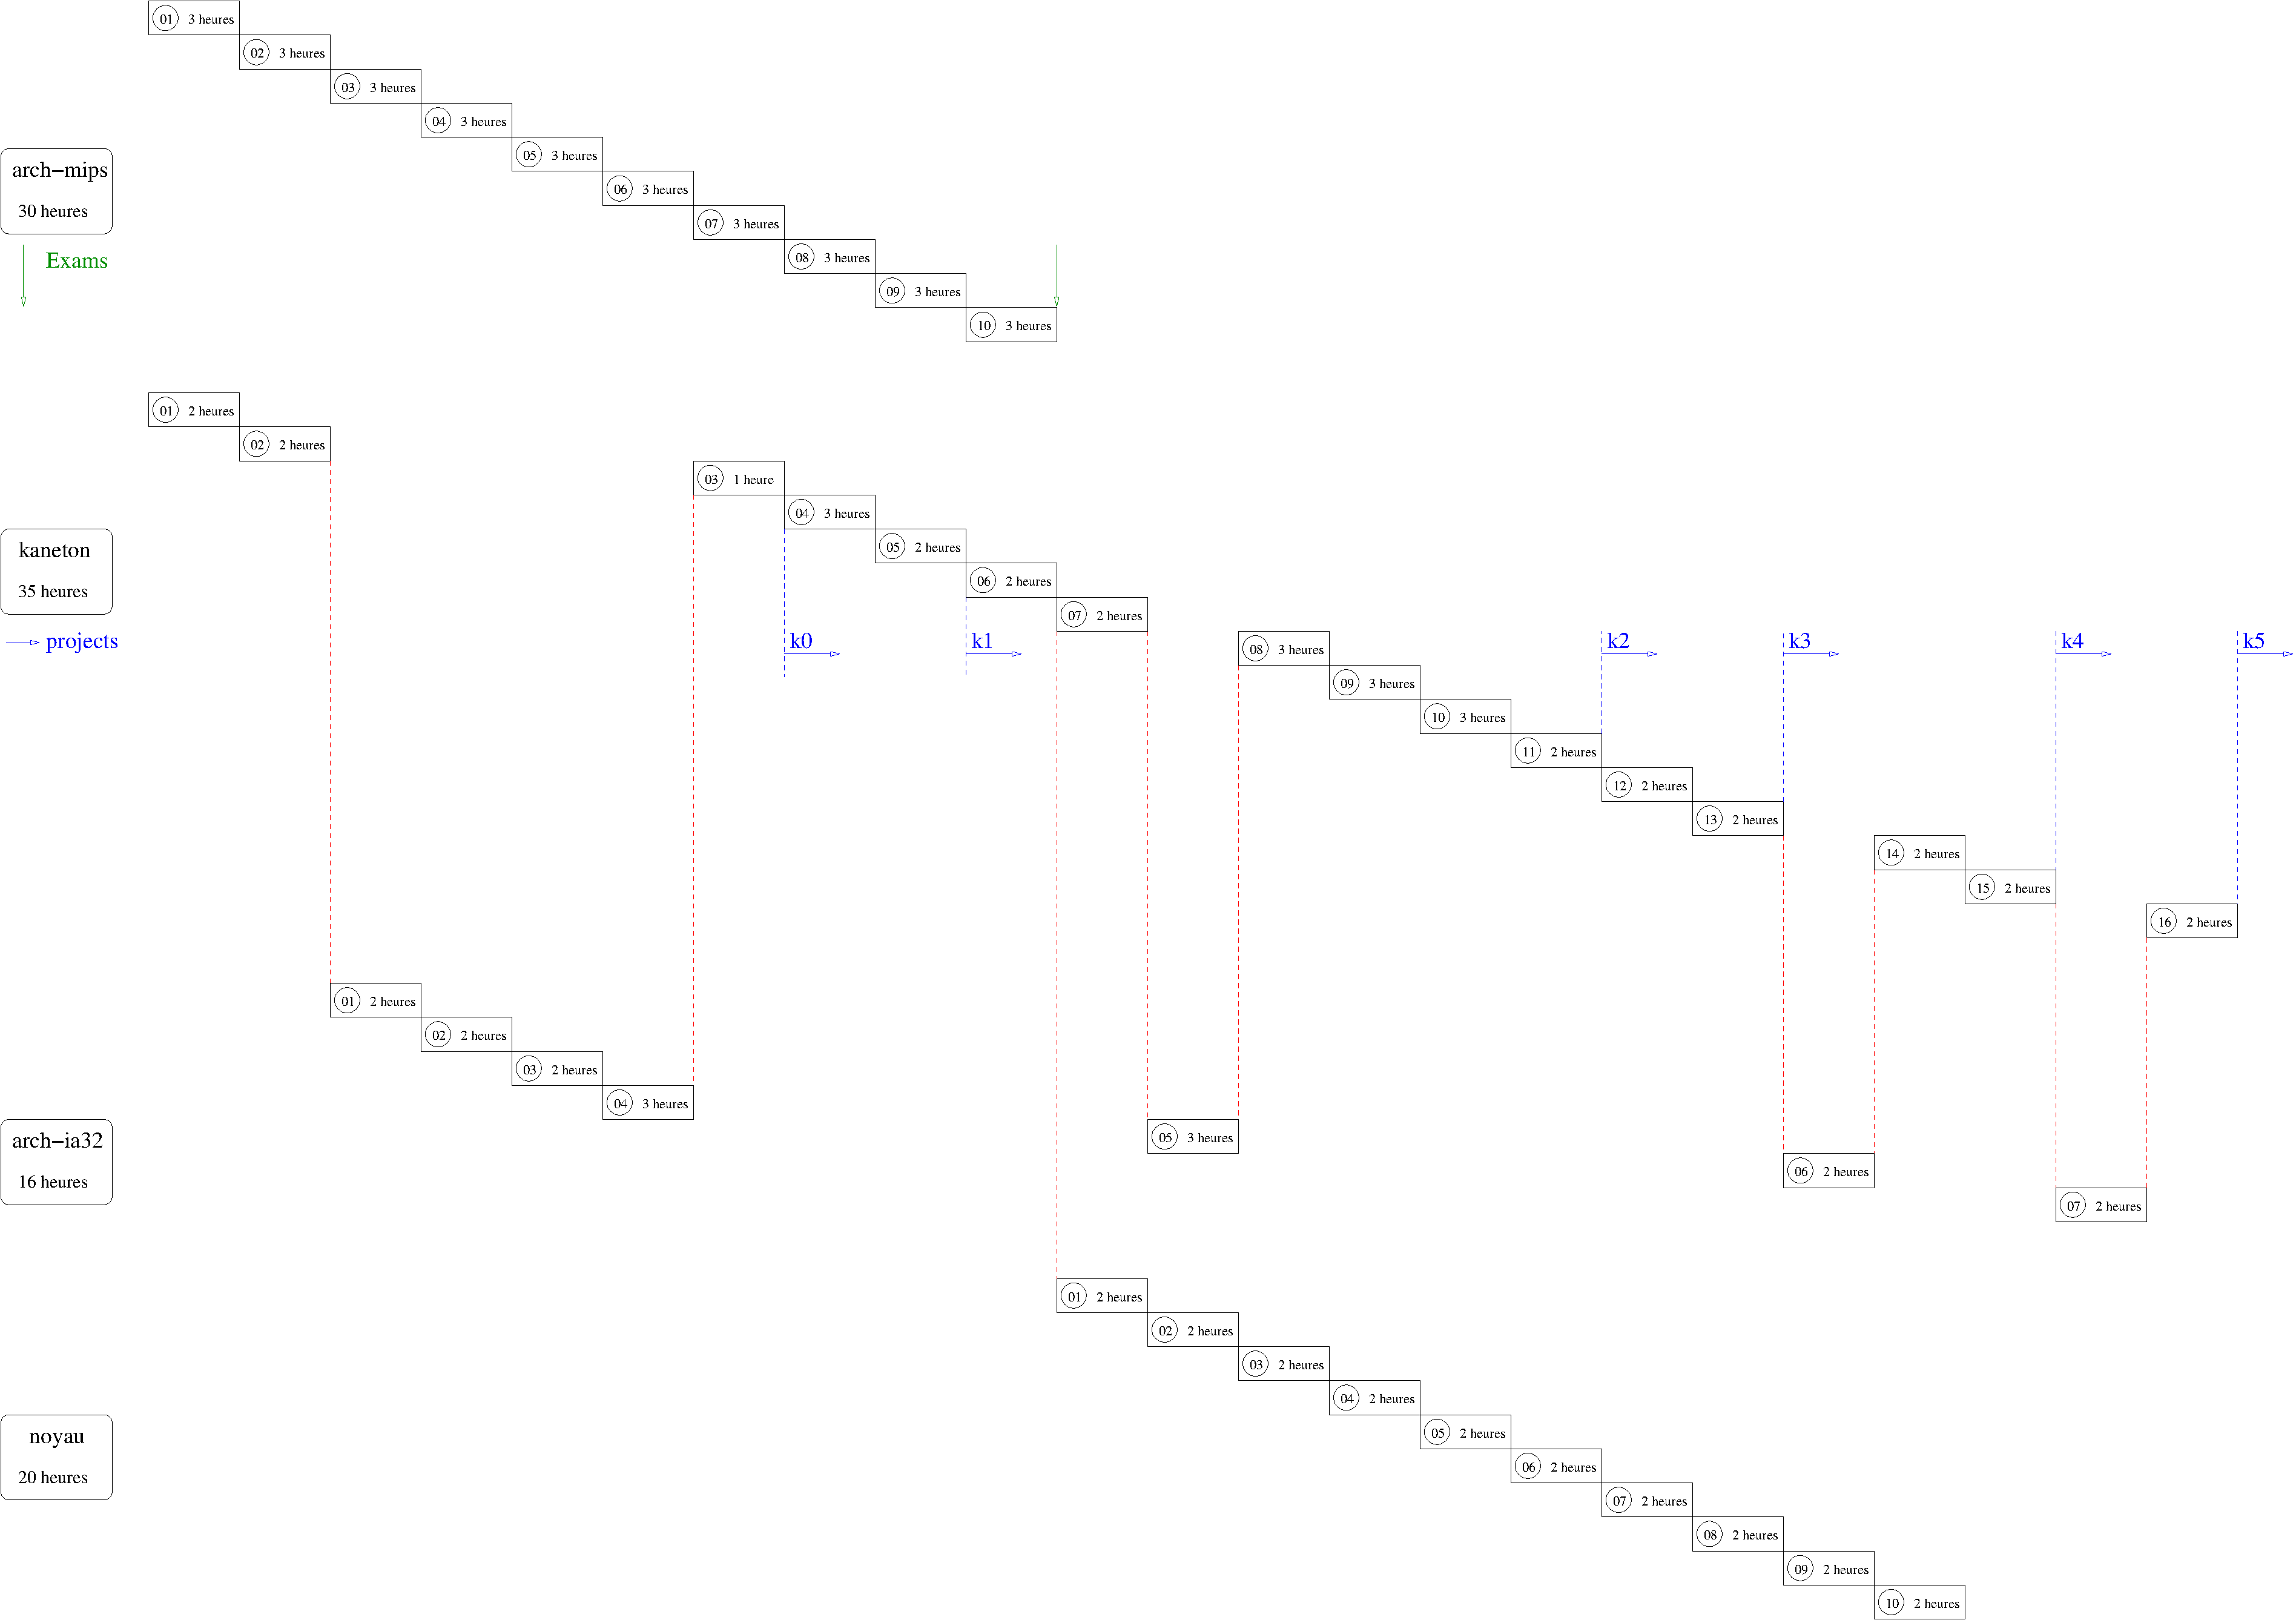
\includegraphics[angle=-90,scale=0.35]{figures/schedule.pdf}}
%\end{figure}

\end{document}
